\documentclass[paper=a4, fontsize=11.0pt, abstractoff, DIV12]{scrartcl}
\usepackage[utf8]{inputenc}
\usepackage[ngerman]{babel} % deutsche Rechtschreibung

\usepackage{graphicx} % Grafiken einbinden
\usepackage{amsmath} % AMS! Wichtig!
\usepackage{amsfonts} % mehr AMS
\usepackage{amssymb} % noch viel mehr
\usepackage[amssymb]{SIunits} % Einheiten anständig setzen
\usepackage{bbm} % fetter gedrucktes verfügbar machen, z.B. \mathbbm{1} = Eins mit Doppelstrich
\usepackage[Euler]{simpleMath}
\usepackage{tikz}
\usepackage{hyperref}
\usepackage{booktabs}
\hypersetup{colorlinks,
            breaklinks=true,
            linkcolor=black,
            urlcolor=black,
            citecolor=black,
            bookmarksnumbered,
            pdfauthor={Alexander Eberspächer},
            pdftitle={Seminar Theoretische Physik}}

\title{Dynamik kontinuierlicher Systeme}
\author{Alexander Eberspächer}
\date{\today}

\newcommand{\LD}{\ensuremath{\mathcal{L}}}
\newcommand{\HD}{\ensuremath{\mathcal{H}}}
\newcommand{\ti}{\ensuremath{t_\mathrm{i}}}
\newcommand{\tf}{\ensuremath{t_\mathrm{f}}}

\begin{document}
\maketitle
\begin{abstract}
Als Ergänzung zur Vorlesung wird kurz vorgestellt, wie sich eine dynamische
Theorie kontinuierlicher Systeme als Grenzfall einer Theorie diskreter
Systeme ergibt. Wir wollen anhand von Beispielen die Grundzüge des
Formalismusses sogenannter \emph{Feldtheorien} kennenlernen.\\[0.5ex]
Literatur: Scheck \cite{Scheck} und José\&Saletan \cite{JoseSaletan}
\end{abstract}

\section{Einleitung - Mechanik diskreter Systeme $\to$ Mechanik der Kontinua}

Die Mechanik diskreter Systeme, wie sie bisher in der Vorlesung besprochen
wurde, kommt immer mit \emph{endlich} vielen Freiheitsgraden aus. Die
\emph{dynamischen Variablen} sind die Größen $q_i(t)$ und $\dot{q}_i(t)$
(beziehungsweise $p_i(t)$ statt $\dot{q}_i(t)$ in der Hamilton-Mechanik).
Die Zeit $t$ spielte die Rolle eines Parameters. Denken wir beispielsweise
an die große Teilchenzahl in einem Festkörper, so erscheint es angemessen,
einen Übergang auf unendlich viele Freiheitsgrade vorzunehmen. Statt der
$q_i(t)$ werden die sogenannten Feldvariablen $\varphi(\vec x, t)$ von
Bedeutung sein. Die Orte werden damit von dynamischen Variablen zu
kontinuierlichen Parametern degradiert und damit symmetrisch zur Zeit
behandelt. Den Übergang wollen wir an der sogenannten linearen Kette
verstehen. Die Diskussion ist in wesentlichen Teilen Schecks Buch
\cite{Scheck} entnommen.

\section{Die lineare Kette}

\subsection{Das System}

Wir betrachten $N$ harmonisch gekoppelte identische Federschwinger, die
entlang der Kette schwingen können (longitudinale Schwingungen):
\begin{center}
    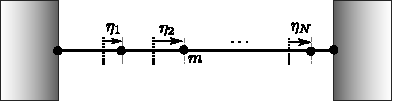
\includegraphics[width=0.5\textwidth]{Kette.pdf}
\end{center}
Die Auslenkungen aus den jeweiligen Ruhelagen $x_{0,i}$ bezeichnen wir mit
\begin{equation}
\eta_i(t) = x_i(t) - x_{0,i}\,.
\end{equation}
Damit schreiben wir für die kinetische und die potentielle Energie
\begin{align}
T &= \sum\limits_{i=1}^{N} \frac{1}{2}m\dot{\eta}_{i}^2\,,\\
V &= \sum\limits_{i=1}^{N} \frac{1}{2}D\left(\eta_{i+1}-\eta_i\right)^2-\frac{1}{2}D\left(\eta_1^2+\eta_N^2\right)\,.
\end{align}
Die letzten Terme in der potentiellen Energie entsprechen dabei dem Anfang
und dem Ende der Kette. Nutzen wir als Randbedingung, dass die äußeren Massen
fest mit der Wand verbunden sind und in der Ruhelage verharren, so können wir
für die potentielle Energie
\begin{equation}
V = \sum\limits_{i=1}^{N-1} \frac{1}{2}D\left(\eta_{i+1}-\eta_i\right)^2
\end{equation}
schreiben. Als Lagrange-Funktion $L=T-V$ ergibt sich dann mit der Abkürzung
$\omega_0^2 = D/m$
\begin{equation}
L =\frac{1}{2}m\sum\limits_{j=0}^{N}\left[\dot{\eta}_j^2 -\omega_0^2(\eta_{j+1}-\eta_j)^2 \right]\,.
\end{equation}
Als Euler-Lagrange-Gleichung für die Größe $\eta_i(t)$ ergibt sich
\begin{equation}
\ddot{\eta}_j =\omega_0^2(\eta_{j+1}-\eta_j) - \omega_0^2(\eta_{j}-\eta_{j+1})\qquad j=1\dots N\,.
\label{eq:BewGl}
\end{equation}
Prinzipiell könnten wir an dieser Stelle wie besprochen Normalfrequenzen und
-schwingungen gemäß unserem ``Kochrezept'' bestimmen, allerdings wollen wir
erst den Übergang zum schwingenden Kontinuum vollziehen.

Man beachte, welchen Status die einzelnen Größen im Rahmen dieser
Punktmechanik haben: wir haben mit $N$ abzählbaren Freiheitsgraden zu tun.
Die $\eta_j$ und die Geschwindigkeiten $\dot\eta_j$ (oder die Impulse $p_j$)
sind die dynamischen Variablen.

\subsection{Übergang zum Kontinuum und der Begriff des \emph{Feldes}}

Der Übergang zum Kontinuum bedeutet, $N\to\infty$ gehen zu lassen. Der
Abstand $d$ zwischen zwei Massen geht dann $\to 0$. Der Übergang soll derart
vollzogen werden, dass die Massendichte $\rho$ konstant bleibt.

Die interessante Größe ist dann die Auslenkung $\phi(x, t)$. Da $x$ und $t$
kontinuierliche Größen sind, haben wir es bei den Auslenkungen $\phi$ mit
\emph{unendlich vielen} Freiheitsgraden zu tun! Sowohl die Zeit $t$ als auch
der Ort haben dann die Rolle von Parametern. Die Größe $\phi$ nennt man ein
\emph{Feld}. Unser Ziel ist es, den bekannten Lagrange-Formalismus für
Felder zu formulieren.

Zunächst betrachten wir an den diskreten Orten $x_j = jL/N+1$ die Feldgröße
\begin{equation}
\phi\left(x=\frac{jL}{N+1}, t\right) = \eta_j(t)\,.
\end{equation}
Die Zeitableitungen
\begin{equation}
\firstpderiv{}{t}\phi\left(x=\frac{jL}{N+1}, t\right) = \dot\eta_j(t)
\label{eq:ZeitAbl}
\end{equation}
brauchen wir später. Die Differenzen $\eta_{j+1}-\eta_j$ aus der
Bewegungsgleichung \eqref{eq:BewGl} schreiben wir als Ableitung
\begin{align}
\eta_{j+1}-\eta_j &=\phi\left(x=\frac{(j+1)L}{N+1}, t\right) - \phi\left(x=\frac{jL}{N+1}, t\right)\nonumber\\
&=\left.\firstpderiv{\phi}{x}\right\vert_{x=jd+d/2}d\,.
\end{align}
Um diese Umschreibung zu verstehen, erinnern wir uns daran, wie man die
Ableitung $f'(x)$ als (zentralen) Differenzenquotienten
\begin{equation*}
f'(x) = \frac{f(x+\epsilon/2) - f(x-\epsilon/2)}{\epsilon}
\end{equation*}
schreiben kann. Analog zur ersten Umschreibung können wir auch die zweite
Differenz, die wir für die Bewegungsgleichung brauchen, durch eine Ableitung
ausdrücken:
\begin{align}
\eta_{j}-\eta_{j-1} &= \phi\left(x=\frac{jL}{N+1}, t\right) - \phi\left(x=\frac{(j-1)L}{N+1}, t\right)\nonumber\\
&=\left.\firstpderiv{\phi}{x}\right\vert_{x=jd-d/2}d\,.
\end{align}
Für die Bewegungsgleichungen benötigen wir
\begin{align}
(\eta_{j+1} - \eta_j) - (\eta_j-\eta_{j-1}) &= \left[\left.\firstpderiv{\phi}{x}\right\vert_{x=jd+d/2} - \left.\firstpderiv{\phi}{x}\right\vert_{x=jd-d/2}\right]d\nonumber\\
&=\left.\secondpderiv{\phi}{x}\right\vert_{x=jd} d^2\,.
\end{align}
Dieses Ergebnis zusammen mit einer weiteren Zeitableitung von
\eqref{eq:ZeitAbl} setzen wir in die Bewegungsgleichung \eqref{eq:BewGl} ein
und erhalten
\begin{equation}
\secondpderiv{\phi}{t} = \omega_0^2d^2\secondpderiv{\phi}{x}\,.
\end{equation}
Im Limes $d \to 0$ strebt der Quotient $d/m$ gegen die reziproke
Längenmassendichte $1/\rho$. Aus $Dd$ wird das Elastizitätsmodul $E$. Wir
schreiben dann den Koeffizienten auf der rechten Seite um zu
\begin{equation}
\omega_0^2d^2 = \frac{Dd^2}{m} = \frac{E}{\rho} =: v^2\,,
\end{equation}
was die bekannte Ausbreitungsgeschwindigkeit von Schallwellen in elastischen
Medien ist. Die ``Bewegungsgleichung'' für die Feldgröße $\phi(x,t)$ ist dann
die bekannte \emph{Wellengleichung}
\begin{equation}
\secondpderiv{\phi}{t} = v^2\secondpderiv{\phi}{x}\,.
\label{eq:Wellengleichung}
\end{equation}
Nach diesem etwas mühseligen Übergang zum Kontinuum stellt sich nun die Frage,
was aus der Lagrange-Funktion $L$ wird.

\subsection{Lagrange-Funktion für das Kontinuum}

Im Übergang $N\to\infty$ geht $d\to \dd x$. Die Summe $\sum d$ wird zum
Integral $\int\!\dd x$ und die Masse $m$ ersetzen wir zunächst durch $\rho d$.
Für den Term $m\omega_0^2 (\eta_{j+1}-\eta_j)^2$ in der Lagrange-Funktion
schreiben wir
\begin{align}
m\omega_0^2 (\eta_{j+1}-\eta_j)^2 &= \rho d \omega_0^2\left(\firstpderiv{\phi}{x}\right)^2d^2\nonumber\\
&= \rho d v^2 \left(\firstpderiv{\phi}{x}\right)^2\,.
\end{align}
Ersetzen wir noch die Zeitableitung nach Gleichung \eqref{eq:ZeitAbl}, so
bekommen wir als Lagrange-Funktion
\begin{equation}
L = \int\!\dd x\,\underbrace{\frac{\rho}{2}\left[\left(\firstpderiv{\phi}{t}\right)^2 - v^2\left(\firstpderiv{\phi}{x}\right)^2 \right]}_{=:\LD}\,.
\label{eq:LDKette}
\end{equation}
Die Lagrange-Funktion $L$ berechnet sich wie ein Integral über eine Dichte,
weshalb der Integrand $\LD$ auch die \emph{Lagrange-Dichte} heißt. Allgemein
darf $\LD$ eine Funktion der Feldgrößen und deren Ableitungen sowie von Ort
und Zeit sein:
\begin{equation}
\LD = \LD(\phi, \partial_x \phi, \partial_t \phi, x, t)\,.
\end{equation}
Wir stellen nun nochmal kurz Punktteilchenmechanik und Feldtheorie gegenüber:
\begin{center}
\begin{tabular}{c c}
diskrete Systeme & kontinuierliche Systeme\\
\toprule
$q_i$ & $\phi(x,t)$\\
$\dot q_i$ & $\partial_x\phi, \partial_t\phi$\\
$t$ & $x, t$\\
\bottomrule
\end{tabular}
\end{center}
Es stellt sich nun die Frage, wie sich aus einer gegebenen Lagrange-Dichte
direkt ``Bewegungsgleichungen'' für die Felder ableiten lassen.

\section{Lagrange-Formalismus für kontinuierliche Systeme}

\subsection{Hamiltonsches Prinzip für Felder}

Genau wie in der Punktteilchenmechanik können wir Euler-Lagrange-Gleichungen
auch für Felder ableiten, indem wir das Hamiltonsche Prinzip verwenden. Wir
beschränken uns hier auf eine Raum- und eine Zeitdimension. Eine
Verallgemeinerung ist problemlos möglich.

Wir bilden zunächst wie bereits bekannt das Wirkungsfunktional
\begin{equation}
S[\phi] = \int\!\dd t \,L = \int\!\dd t\int\!\dd x\,\LD\,.
\end{equation}
Dann fordern wir, dass für physikalische Felder die Wirkung extremal ist:
\begin{equation}
\delta S = 0\,.
\label{eq:HamPrinzip}
\end{equation}

Im Folgenden bezeichnen Punkte zeitliche und Striche räumliche Ableitungen.
Wir fordern von der Variation
\begin{equation}
\delta S[\phi] = \int\limits_{\ti}^{\tf}\!\dd t\int\!\dd x\,\left[\firstpderiv{\LD}{\phi}\delta\phi+\firstpderiv{\LD}{\dot{\phi}}\delta\dot{\phi}+\firstpderiv{\LD}{\phi'}\delta \phi' \right]\,,
\end{equation}
dass Sie an Anfangs- und Endzeitpunkten $\ti$ beziehungsweise $\tf$
verschwindet. Außerdem sollen Variation und Ableitung vertauschen:
\begin{align}
\delta\dot{\phi} &= \partial_t\delta\phi\,,\\
\delta\phi' &= \partial_x\delta\phi\,.
\end{align}
Nun fordern wir zusätzlich noch, dass die Variation auch auf den Rändern des
$x$-Integrations\-in\-ter\-valls verschwindet. Dann schieben wir mit Hilfe
von partieller ($x$-)Integration die Ableitungen in den Ausdrücken
$\partial_t\delta\phi$ und $\partial_x\delta\phi$ auf die Lagrange-Dichte
und erhalten -- nachdem wir die Randterme Null gesetzt haben
\begin{equation}
\delta S[\phi] = \int\limits_{\ti}^{\tf}\!\dd t\int\!\dd x\,\left[\firstpderiv{\LD}{\phi} - \firstpderiv{}{t}\firstpderiv{\LD}{\dot{\phi}} - \firstpderiv{}{x}\firstpderiv{\LD}{\phi'} \right]\delta{\phi}\,.
\end{equation}
Nach dem Hamiltonschen Prinzip \eqref{eq:HamPrinzip} soll der gesamte Ausdruck
verschwinden -- da aber die Variation $\delta\phi$ beliebig ist, muss der
Ausdruck in eckigen Klammern selbst gleich Null sein. Wir erhalten damit die
Euler-Lagrange-Gleichung
\begin{equation}
\firstpderiv{\LD}{\phi} - \firstpderiv{}{t}\firstpderiv{\LD}{\dot{\phi}} - \firstpderiv{}{x}\firstpderiv{\LD}{\phi'} = 0\,.
\label{eq:ELG}
\end{equation}

Wir wollen damit nochmal direkt aus der Lagrange-Dichte der gekoppelten
Schwinger aus Gleichung \eqref{eq:LDKette} die Wellengleichung ableiten.
Die Lagrange-Dichte hängt nicht von $\phi$ selbst ab. Damit ist
\begin{equation}
\firstpderiv{\LD}{\phi} = 0\,.
\end{equation}
Die anderen benötigten Terme für die Euler-Lagrange-Gleichung sind
\begin{align}
-\firstpderiv{}{x}\firstpderiv{\LD}{(\partial_x\phi)} &= +\rho v^2 \firstpderiv{}{x}\partial_x\phi =\rho v^2 \partial_x^2\phi\,,\\
-\firstpderiv{}{t}\firstpderiv{\LD}{(\partial_t\phi)} &= -\rho \firstpderiv{}{t}\partial_t\phi = -\rho \partial_t^2\phi\,.
\end{align}
Setzen wir das alles in die Euler-Lagrange-Gleichung \eqref{eq:ELG} ein, so
erhalten wir  erneut die Wellengleichung \eqref{eq:Wellengleichung}.

\subsection{Verallgemeinerung auf mehr Raumdimensionen und mehrere Felder}

Die Verallgemeinerung auf mehr Raumdimensionen bereitet keine Probleme --
aus der partiellen Ortsableitung $\partial_x\phi$ werden die drei
Komponenten des Gradienten $\nabla \phi = \partial_i\phi\,(i=1\dots3)$. Aus
$\firstpderiv{}{x}\firstpderiv{\LD}{(\partial_x\phi)}$ wird die Summe
\begin{equation}
\firstpderiv{}{x}\firstpderiv{\LD}{(\partial_x\phi)} \to \sum\limits_{i=1}^{3} \firstpderiv{}{x^i}\firstpderiv{\LD}{(\partial_i \phi)}\,.
\end{equation}
Unter Verwendung der Einsteinschen Summenkonvention kann das Summenzeichen
auch weggelassen werden.

In der bisherigen Ausführung ist die Rolle von Raum und Zeit in unserer
Theorie schon wesentlich viel symmetrischer als in der
Punktteilchenmechanik. Einen Schritt weiter können wir in der Notation
gehen, indem wir die Zeit und die drei Orte als die vier Komponenten des
Vektors
\begin{equation}
x = \left(x^0, x^1, x^2, x^3\right) = (t, x, y, z)
\end{equation}
auffassen.\footnote{Um die selben Einheiten für die Zeitkomponente und die
Ortskomponenten zu benutzen, könnten wir die Zeit noch mit einer
Geschwindigkeit $c$ multiplizieren. Wir setzen diese hier $c=1$.} Im
Folgenden sollen griechische Indizes über die vier Werte von $0$ bis $3$
laufen.

Wir können unseren Formalismus auch auf mehrere Felder verallgemeinern --
die Felder indizieren wir mit dem Index $I$ durch. Die allgemeinste
Lagrange-Dichte ist also kompakt geschrieben
\begin{equation}
\LD = \LD(\phi_I, \partial_\mu\phi_I, x)\,.
\end{equation}
Für jedes Feld $\phi_I$ können wir dann als Euler-Lagrange-Gleichung
\begin{equation}
\firstpderiv{}{x^\mu}\firstpderiv{\LD}{(\partial_\mu\phi_I)} - \firstpderiv{\LD}{\phi_I} = 0
\end{equation}
schreiben. Der erste Term ist dabei eine Summe über $\mu = 0\dots3$.

\subsection{*Anmerkungen zur Lagrangedichte und deren Struktur}

\begin{itemize}
    \item Man nennt eine physikalische Theorie \emph{lokal}, wenn in der
    Lagrange-Dichte alle Felder an den selben Raumzeit-Punkten eingehen.

    \item Relativistische Feldtheorien sind möglich -- dazu benutzt man den
    passenden metrischen Tensor $g_{\mu\nu}$ und baut Lagrange-Dichten, in
    denen die einzelnen Terme sich korrekt wie Skalare unter
    Lorentz-Transformationen verhalten.

    \item Die Lagrange-Dichte einer Theorie ist nicht eindeutig. Analog zu
    \begin{equation}
    L \to L' = L + \firstderiv{f}{t}\,,
    \end{equation}
    was in der Punktteilchenmechanik auf identische Bewegungsgleichungen
    führte, können wir in einer Feldtheorie eine Vierer-Divergenz addieren:
    \begin{equation}
    \LD \to \LD' = \LD + \partial_\nu f^\nu(x^\mu)\,,
    \end{equation}
    woraus die selben Bewegungsgleichungen resultieren.

    \item Wie in der Punktteilchenmechanik gibt es auch eine
    feldtheoretische Version des Noether-Theorems. Ist $\LD$ invariant unter
    einer kontinuierlichen Symmetrie, so existieren Kontinuitätsgleichungen
    für Flussgrößen.
\end{itemize}

\subsection{*Hamiltonsche Formulierung -- ein Anriss}

Wenn eine Lagrange-Dichte $\LD$ nicht von der Feldfunktion $\psi_I$ abhängt,
dann lautet die $I$-te Euler-Lagrange-Gleichung (diejenige für Feld $\psi_I$)
\begin{equation}
\firstpderiv{}{x^\mu} \firstpderiv{\LD}{(\partial_\mu\LD)} = 0\,.
\end{equation}
Diese vier (Summenkonvention!) Gleichungen zusammen beschreiben einen Fluss,
für den die Kontinuitätsgleichung
\begin{equation}
\partial_0 j^0 + \nabla \cdot\vec j = 0
\end{equation}
gilt. Die Größe $j^\mu=(j^0, \vec j)$ ist hierbei
\begin{equation}
j^\mu = \firstpderiv{\LD}{(\partial_\mu\psi_I)}\,.
\end{equation}
Eine analoge Situation hat man in der Punktteilchenmechanik, wenn $L$ nicht
von $q_i$ abhängt. Der zu $q_i$ konjugierte Impuls $p_i = \partial
L/\partial\dot q_i$ ist dann erhalten.

Wollen wir nun durch diese Analogiebetrachtung kanonisch konjugierte Impulse
in eine Feldtheorie einführen, so haben wir das Problem, dass es zu jedem
Feld $\psi_I$ \emph{vier} Impulse $j^\mu$ gäbe! Deswegen definieren wir den
Impuls als
\begin{equation}
\pi_I(x) := \firstpderiv{\LD}{(\partial_0 \psi_I)}\,.
\end{equation}
Man beachte die Zeitableitung (\emph{eine} Ableitung statt \emph{vieren!}).

Analog zur Legendre-Transformation $H := \dot q_i p_i - L$ der
Punktteilchenmechanik definieren wir das Hamiltonfunktional
\begin{equation}
H = \int\!\dd^3 x\,(\partial_0\psi_I)\pi_I - L = \int\!\dd^3x\underbrace{\left[(\partial_0\psi_I)\pi_I - \LD\right]}_{=:\HD}\,,
\end{equation}
wobei die Hamiltondichte $\HD$ eine Energiedichte ist. Für die kanonischen
Gleichungen der Feldtheorie sei auf die Literatur verwiesen \cite
{JoseSaletan}.

\section{Beispielsysteme/-feldtheorien}

\subsection{Gekoppelte Pendel und die ``Sine-Gordon''-Gleichung}

Ein System aus $N$ gekoppelten Pendeln der Länge $l$ und Masse $m$ soll
transversal zur Verbindungslinie schwingen können.
\begin{center}
    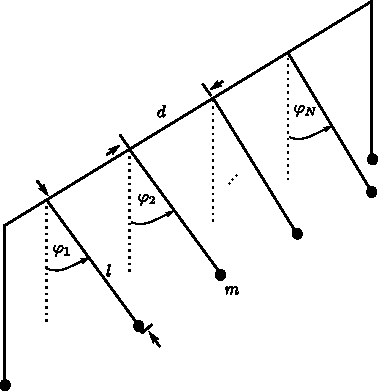
\includegraphics[width=0.375\textwidth]{Pendel.pdf}
\end{center}
Die einzelnen Pendel seien untereinander auf einem Torsionstab so gekoppelt,
dass das zwischen dem $i$-ten und dem $i+1$-ten Pendel das Drehmoment
$-k(\varphi_{i+1} - \varphi_i)$ wirkt. Wir stellen uns wie gehabt an den
Enden des Stabes zwei starr mit der Wand verbundene Pendel mit den Indizes
$0$ und $N+1$ vor und schreiben dann für die kinetische Energie
\begin{equation}
T = \frac{1}{2}ml^2\sum\limits_{j=0}^{N+1}\dot\varphi_j^2
\end{equation}
und für die potentielle Energie
\begin{equation}
V = mgl\sum\limits_{j=0}^{N+1}(1-\cos(\varphi_j)) + \frac{1}{2}k\sum\limits_{j=0}^{N}\left(\varphi_{j+1} - \varphi_j\right)^2\,.
\end{equation}
Die erste Summe in $V$ beschreibt das Potential durch die (äußere)
Gravitationskraft, die zweite Summe das Potential durch die (internen)
harmonischen Torsionskräfte. Die Euler-Lagrange-Gleichung für ein inneres
Pendel $j$ ist dann
\begin{equation}
\ddot\varphi_{j} - \omega_0^2\left[(\varphi_{j+1} - \varphi_{j}) - (\varphi_{j}-\varphi_{j-1})\right] + \omega_1^2\sin(\varphi_j) = 0\,,
\end{equation}
wobei die beiden Abkürzungen
\begin{align}
\omega_0^2 &:= \frac{k}{ml^2}\nonumber\,\\
\omega_1^2 &:= \frac{g}{l}\nonumber
\end{align}
benutzt worden sind. Der Sinus-Term macht die Gleichung \emph{nichtlinear}.

Mit dem Pendelabstand $d$ hat die Kette die Länge $L=(N+1)d$. Im
Grenzübergang $N\to\infty$, $d\to 0$ erhalten wir auch hier wieder ein
kontinuierliches System. Die Winkel $\varphi_j$ werden durch die Feldgrößen
$\varphi(x,t)$ ersetzt. Für mehr Details zum Übergang vergleiche \cite
{Scheck}. Mit $v^2:=\omega_0^2 d^2$ erhalten wir die
``Sinus-Gordon-Gleichung'' oder englisch die ``Sine-Gordon
equation''\footnote{Ein Reim auf die bekannte Klein-Gordon-Gleichung}
\begin{equation}
\partial_t^2\varphi - v^2\partial_x^2\varphi + \omega_1^2\sin(\varphi) = 0\,.
\end{equation}
Diese Gleichung ergibt sich aus der Lagrange-Dichte
\begin{equation}
\LD = \frac{1}{2}\rho l^2\left[ (\partial_t \varphi)^2 - v^2 (\partial_x \varphi)^2 - \omega_1^2(1-\cos(\varphi))\right]\,.
\end{equation}
Die Sinus-Gordon-Gleichung hat interessante Soliton-Lösungen.

\subsection{*Komplexe Felder: das Schrödingerfeld}

Als Fingerübung wollen wir die Euler-Lagrange-Gleichungen für das
Schrödingerfeld
\begin{equation}
\LD =\frac{\ii\hbar}{2}\left[\psi^*\dot\psi - \dot{\psi}^*\psi \right] - \frac{\hbar^2}{2m}\nabla\psi^*\cdot\nabla\psi - V(\vec r)\psi^*\psi
\end{equation}
ableiten. Wir haben es hier mit einem \emph{komplexen} Feld $\psi$ zu tun.
Dieses lässt sich -- analog zur Zerlegung $\psi = \Real\psi + \ii\Imag\psi$
in (von einander unabhängige) Real- und Imaginärteile -- durch die beiden
unabhängigen Felder $\psi$ und $\psi^*$ behandeln. Es gilt selbstverständlich
\begin{align*}
\Real\psi &= \frac{1}{2}\left(\psi + \psi^*\right)\,,\\
\Imag\psi &= \frac{1}{2}\left(\psi - \psi^*\right)\,.
\end{align*}
Wir leiten nun die Euler-Lagrange-Gleichung für das Feld
$\psi^*$ ab. Es ist
\begin{align*}
\firstpderiv{\LD}{(\psi^*)} &= \frac{\ii\hbar}{2}\dot\psi-V(\vec r)\,,\\
-\firstpderiv{}{t}\firstpderiv{\LD}{(\dot\psi^*)} &= \frac{\ii\hbar}{2}\dot\psi\,,\\
-\nabla\firstpderiv{\LD}{(\nabla\psi^*)} &= +\frac{\hbar^2}{2m}\nabla\cdot\nabla\psi = +\frac{\hbar^2}{2m}\Delta\psi\,.
\end{align*}
Damit ist die Euler-Lagrange-Gleichung
\begin{equation}
\ii\hbar \dot\psi =\left[ -\frac{\hbar^2}{2m}\Delta + V(\vec r)\right]\psi
\end{equation}
identisch der Schrödinger-Gleichung! Man beachte, dass damit nicht die
komplette Quantenmechanik abgeleitet ist -- diese besteht neben der
Schrödingergleichung auch noch aus der Interpretation, die wir im Rahmen
dieser Fingerübung nicht erhalten\dots

\bibliographystyle{ieeetr}

\bibliography{Mechanik-Kontinua}

\end{document}
